\documentclass[12pt, oneside]{article}   	% use "amsart" instead of "article" for AMSLaTeX format
\usepackage{geometry}                		% See geometry.pdf to learn the layout options. There are lots.
\geometry{letterpaper}                   		% ... or a4paper or a5paper or ... 
%\geometry{landscape}                		% Activate for for rotated page geometry
%\usepackage[parfill]{parskip}    		% Activate to begin paragraphs with an empty line rather than an indent
\usepackage{graphicx}				% Use pdf, png, jpg, or eps� with pdflatex; use eps in DVI mode
\usepackage{amsmath}
\usepackage{mathtools}
								% TeX will automatically convert eps --> pdf in pdflatex		
\usepackage{amssymb}
\numberwithin{equation}{section}
\numberwithin{table}{section}
\usepackage{color}
\usepackage[toc,page]{appendix}
\usepackage[hypcap]{caption}
\usepackage{caption}
% Set Margin Sizes
%%%%%%%%%%%%%%%%%%%%%%%%%%%
 \geometry{
 a4paper,
 left= 30mm,
 right= 20mm,
 top= 25mm,
 bottom= 25mm,
 }
%%%%%%%%%%%%%%%%%%%%%%%%%%%
  
% Set Line Spacing
%%%%%%%%%%%%%%%%%%%%%%%%%%%
\usepackage{setspace}
\singlespacing
%\onehalfspacing
%\doublespacing
%\setstretch{1.1}
%%%%%%%%%%%%%%%%%%%%%%%%%%%

\title{Scripsie: State Estimation \& Observation}
\author{Aidan Landsberg}
\date{\today}							% Activate to display a given date or no date
\pagenumbering{roman}
\begin{document}
\maketitle
\newpage
\tableofcontents
\newpage

\listoffigures
\listoftables
%\listofequations

\newpage
\pagenumbering{arabic}
%%%%%%%%%%%%%%%%%%%%%%%%%%%%%%%%%%%%%%%%%%%%%%%%%%%%%%%%%%%%%%%%%%%%%%%%%%
\section{Single Camera Simultaneous Localisation and Mapping }
The ultimate goal of the approach presented here, is to obtain a probabilistic three dimensional (3D) map of features, representing at every time instance, the estimates of both the state of the camera as well as the positions of every feature observed. These features of interest are more commonly referred to as \textit{landmarks} and the aforementioned terms will, from hereon in, be used synonymously.  Most importantly though, the map is to contain the \textit{uncertainty} associated with each of the aforementioned estimates.\\The process regarding the construction of this map of features is to be implemented through the use of an (Extended) Kalman filter. The map initially, completely void of any landmarks, is recursively updated according to the subsequent fusions of both predictions and measurements presented to the Kalman filter. As new (potentially interesting) features are observed, the state estimates of both the camera as well as the landmarks are both updated - augmenting the state vector with additional features (if indeed they are observed) while deleting any landmarks that are no longer of interest. In order to obtain the best possible result, the algorithm should strive to obtain a sparse set of higher-quality landmarks rather than a dense set of ordinary landmarks within the environment.   \\ 
Before continuing, it is important to consider and understand the notation used in the sections that follow. Two separate coordinate systems are to be considered, namely the \textit{fixed} inertial reference frame system $W$ and the cameras free coordinate frame system, more commonly referred to as the body frame $C$. System variables defined within either of the aforementioned coordinate systems, are from here on in, to be designated a superscript to establish in which coordinate system it may be relevant (e.g. $x^{W}$). Derivatives of parameters are denoted through a dot symbol, second derivates are denoted through a double dot symbol and so forth; for instance the derivative of position $x$ will be denoted as $\dot{x}$ and its second derivative denoted as $\ddot{x}$. Vectors will be printed in bold and non-italics to better distinguish them from scalars. An example can be shown regarding the variable x: $\textbf{x}$ denotes a vector while its scalar counterpart would be represented as \textit{x}. 
%%%%%%%%%%%%%%%%%%%%%%%%%%%%%%%%%%%%%%%%%%%%%%%%%%%%%%%%%%%%%%%%%%%%%%%%%%    
\newpage
\section{Recursive State Estimation}
Probabilistic robotics yields a unique yet fundamental concept at its core, that is: estimating a state through sensor data. Quantities exist that are not directly observable, yet are still able to be obtained through sensor data. Sensors though, obtain limited data regarding certain quantities and most importantly, are affected and often corrupted by \textit{noise}.\\
Recursive state estimation then, seeks to recover state variable from the obtained sensor data bearing in mind the previously mentioned limitations. Probabilistic state estimation algorithms - to be investigated in this section - compute \textit{belief} distributions regarding state variables. The following section will provide a brief, yet concise introduction to these various algorithms. The fundamental concepts, particularly the various techniques associated with the implementation thereof will be addressed.\\\\
The goal of this section is to introduce the fundamental concepts as well as the mathematical and probabilistic principles that form the basis of state estimation in the robotics field of study. Initially, the Bayes Filter; that is the algorithm that forms the basis of all state estimation techniques presented in this paper, will be introduced and formally discussed. Thereafter, the Gaussian Filter family - particularly the Kalman Filter as well as it's variants - are to be introduced, discussed and defined in terms of the context of this paper.   
%%%%%%%%%%%%%%%%%%%%%%%%%%%%%%%%%%%%%%%%%%%%%%%%%%%%%%%%%%%%%%%%%%%%%%%%%%
\subsection{Bayes Filter}
Upon considering probabilistic robotics, a key concept worth describing is the previously mentioned \textit{belief} of a robot. Briefly, the belief represents the robot's understanding regarding the state of it's own dynamics as well as the dynamics of the surrounding environment. This critical concept proves a fundamental basis in probabilistic robotics. The belief can be represented as a conditional probability distribution whereby each possible scenario (state) is a signed a probability (density). Mathematically the belief with regard to a state variable $x_t$ is denoted as follows:
\begin{equation} \label{eq:belief}
bel(x_t) = p(x_t\hspace{0.1cm}|\hspace{0.1cm}z_{1:t},\hspace{0.1cm}u_{1:t}),
\end{equation}
A brief description would yield that the distribution above describes, for a given time instance $t$, a joint density of the robot state as well as the landmark locations \textbf{given} all of the previously recorded observations ${z}_{1:t}$ and control inputs ${u}_{1:t}$.\\
Considering that the state of the robot is constantly updated at every time-step $t$ and that each update is dependent upon the state at the previous time-step, it is essential that the algorithm required be recursive in nature. The \textit{Bayes Filter} algorithm provides precisely such a procedure. The algorithm calculates the belief distribution stated in equation~\ref{eq:belief} from the observation and control data. The table below presents a pseudo-algorithmic interpretation of the Bayes Filter algorithm \textcolor{red}{and is based on the definition as in Probabilistic Robotics...}:

\begin{table}[h]
\begin{center}
\caption{The Bayes Filter Algorithm} \label{tab:BF}
\begin{tabular}{l l l}
\hline
\textbf{Input}: &previous belief $bel(x_{t-1})$, control input/s ${u}_t$, measurement/s ${z}_t$\\ 
\textbf{Output}: &current belief $bel(x_{t})$\\
\hline
\hline
for all $x_t$: \\
1. & $\overline {bel}(x_t)$ = $\int p(x_t\hspace{0.1cm}|\hspace{0.1cm}u_{t},\hspace{0.1cm}x_{t-1})bel(x_{t-1})dx_{t-1}$ \\
2. & ${bel}(x_t)$ = $\eta p(z_t\hspace{0.1cm}|\hspace{0.1cm}x_{t})\overline {bel}(x_t)$ \\
3. &end for. \\
\hline\hline
\end{tabular}
\end{center}
\end{table}%
The recursive nature of the algorithm can thus be seen from table~\ref{tab:BF} above; whereby the belief $\overline {bel}(x_t)$ at the current time $t$ is obtained through initially calculating the belief at the previous time-step $t-1$. The Bayes Filter contains two essential steps: \textit{prediction} (line 1) and \textit{measurement update} (line 2). The prediction step initially processes the control inputs before subsequently predicting the current belief based on the prior belief as well as the probability that the control inputs induce a transition form $x_{t-1}$ to $x_t$. Thereafter, the measurement update seeks to determine the belief in the event that a measurement has been observed that may correct any errors presented in the previous prediction step.\\
The mathematical derivation of the Bayes Filter contains many assumptions and further technicalities. The techniques presented in this paper though, require only a basic comprehension of it's implementation. Furthermore, detailed analysis of the Bayes Filter can be obtained through these sources as well as the appendix \textcolor{blue}{(Probabilistic Robotics, Cyril Stachnis etc.).} \\
\textcolor{red}{This summary is taken from Probabilistic Robotics... Remember to reference.}\\
%%%%%%%%%%%%%%%%%%%%%%%%%%%%%%%%%%%%%%%%%%%%%%%%%%%%%%%%%%%%%%%%%%%%%%%%%%
\newpage
\subsection{Gaussian Filters}
%%%%%%%%%%%%%%%%%%%%%%%%%%%%%%%%%%%%%%%%%%%%%%%%%%%%%%%%%%%%%%%%%%%%%%%%%%
As previously discussed, the Bayes Filter possesses many different derivations and variants thereof. Amongst these derivations, are the \textit{Gaussian filter} family. The basic idea behind a Gaussian filter is that beliefs can be represented as a multivariate Gaussian distributions, represented mathematically as follows:
\begin{equation} \label{eq:normal}
p(x_t)=\cfrac{1}{\sqrt{|2\pi\Sigma|}}\hspace{0.1cm}\text{exp}\hspace{0.1cm}\bigg\{-\frac{1}{2}(x_t-\mu)^T\Sigma^{-1}(x_t-\mu)\bigg\},
\end{equation} 
where the density across the state variable $x_t$ is characterised through two fundamental parameters: The mean $\mu$ and the covariance $\Sigma$. Such a parameterisation whereby a Gaussian is characterised through it's respective mean and covariance is called the \textit{moments parameterisation} (as the mean and covariance represent the first and second order moments respectively). Here from, a number of recursive filter algorithms can be derived, two of which are examined in this paper: the \textit{Kalman Filter} (KF) and it's non-linear counterpart, the \textit{Extended Kalman Filter} (EKF). It is important to realise that both of the aforementioned Filters belong to the same sub-class of filters - namely the Kalman Filter Family - and therefore most of the fundamental concepts and functionality between them are identical. Each Filter is discussed in further detail in the following segments of this section.   
%%%%%%%%%%%%%%%%%%%%%%%%%%%%%%%%%%%%%%%%%%%%%%%%%%%%%%%%%%%%%%%%%%%%%%%%%%
\subsubsection{Kalman Filter}    
Probably the most fundamental (and popular) of all Gassian filter algorithms, is the \textit{Kalman Filter}. The Kalman filter can be briefly described as the algorithm that enables the realisation of many practical recursive estimation systems, including the SLAM problem. It remains a popular, well studied technique for filtering and prediction of linear systems that contains uncertainty - typically uncertainties which are Gaussian in nature. The Kalman filter seeks to describe a belief distribution of a state variable $\textbf{{x}}_t$ as described in equation~\ref{eq:normal}. Subsequently, the state vector $\textbf{{x}}_t$ is modelled by a single multivariate Gaussian distribution with a mean $\mu_t$ and covariance $\Sigma_t$, at each time instance $t$ (while previous time-steps are denoted as $t-1$, $t-2$, etc.). The general implementation as described above though, is only valid provided that the following three properties hold true: 
\begin{enumerate}
\item The state transition model probability - with function $g(\textbf{u}_{t},\hspace{0.1cm}\mu_{t-1})$ - \textbf{must} be a \textit{linear} function with additive Gaussian (process) noise.
\item The observation model probability - with function $h(\bar \mu_t)$ - \textbf{must} be a \textit{linear} function with additive Gaussian (measurement/sensor) noise. 
\item The initial belief $bel(x_0)$ must be normally distributed.
\end{enumerate}
In the context of Simultaneous Localisation and Mapping (SLAM), a Kalman Filter algorithm \textbf{optimally} estimates the state of the robots pose as well as the position of the landmarks within the map, given process and measurement noise.\\
%provided that the state vector $\textbf{\^{x}}_k$, and landmark locations $\textbf{\^{y}}_{n,k}$ are modelled by a single multivariate Gaussian distribution. The system is to be observed at discrete steps in time - denoted by the subscript$k =1, 2,  3, ...$ - where at every individual time-step, it can be influenced by a set of actions. It is assumed that\\  
Moreover, the solution to this specific implementation of the SLAM problem, takes a probabilistic form where the belief with regard to state variable $\textbf{x}_t$ is denoted as shown in equation~\ref{eq:belief}:
\begin{equation}
bel(\textbf{{x}}_t) = p\big(\textbf{{x}}_t\hspace{0.15cm}|\hspace{0.15cm}\textbf{z}_{1:t},\textbf{u}_{1:t}\big),
\end{equation}
%with the aforementioned distribution described at every discrete time instance $t$.\\ A brief description would yield that the distribution above, describes, for a given time instance $t$, a joint density of the robot state as well as the landmark locations \textbf{given} all of the previously recorded observations, $\textbf{z}_{1:t}$ and control inputs, $\textbf{u}_{1:t}$.\\
Like the Bayes Filter, the Kalman filter too is executed in two (sequential) steps: the \textit{prediction step} and the \textit{update step}. Firstly, the prediction step aims to estimate a state into which the system will be transitioned from the previous state estimate ($\mu_{t-1}$, $\Sigma_{t-1}$) as a result of a set of internal and/or external dynamics to the system. These dynamics are typically described through the state transition function $g(\mu_{t}, {\mu}_{t-1})$. Once an estimate is obtained for the transitioned state estimate ($\bar \mu_t$, $\bar \Sigma_t$), a measurement prediction is made in order to provide the expected measurements provided that the system were to find itself within the estimated transitioned state. These measurements are obtained through an observation model which has a function $h(\bar \mu_t)$. Thereafter, an actual measurement, $\textbf{z}_t$ is then obtained through the system sensors in order to determine the actual state of the system ($\mu_t$, $\Sigma_t$). Ultimately, the actual state of the system and the previously predicted state are then compared with one another in order  to obtain the (optimally weighted) \textit{Kalman gain}: This entity yields minimum mean-squared error in the estimate and ultimately provides an optimal trade-off between the measurement and the estimate. Intuitively, the Kalman gain controls how much the systems "trusts" the measurements over the estimate. Each of the aforementioned steps are later discussed in more detail - with reference to implementations specific to this paper. Table~\ref{tab:KF} below, presents a pseudo-algorithmic representation the aforementioned steps. Table~\ref{tab:KF} also incorporates a systematical and mathematical representation for the following system definition of the state transition and the observation models respectively:
\begin{equation}\label{eq:SSmodel}
\begin{split}
g(\textbf{u}_{t}, {\mu}_{t-1}) &:  \textbf{x}_t = \textbf{A}_t\textbf{x}_{t-1} + \textbf{B}_t\textbf{x}_t + \textbf{w}_t\\
h(\bar \mu) &: \textbf{z}_t = \textbf{C}_t\textbf{x}_t + \textbf{v}_t
\end{split}
\end{equation}
where $\textbf{w}_t$ and $\textbf{v}_t$ represent process and sensor noise respectively.
\begin{table}[h]
\begin{center}
\caption{The Kalman Filter Algorithm}\label{tab:KF}
\begin{tabular}{l l l}
\hline
\textbf{Input}: &previous mean $\mu_{t-1}$ and covariance $\Sigma_{t-1}$, control inputs $\textbf{u}_t$, measurements $\textbf{z}_t$\\ 
\textbf{Output}: &mean $\mu_{t}$, covariance $\Sigma_{t}$\\
\hline
\hline
&\textit{Prediction step} \\
\hline
1. & $\bar \mu_{t}$ = $g(\textbf{u}_{t}, \mu_{t-1})$ = $\textbf{A}_t\hspace{0.05cm}\mu_{t-1} + \textbf{B}_t\hspace{0.05cm}\mu_t$ + $\textbf{w}_t$\\
2. & $\bar \Sigma_t = \textbf{A}_t \Sigma_{t-1} \textbf{A}_t^T + R_{w,t}$ \\
\hline
&\textit{Correction step}\\
\hline
3. & $K_t = \bar \Sigma_{t} \textbf{C}_t^T (\textbf{C}_t \bar \Sigma_{t} \textbf{C}_t^T + Q_{v,t})^{-1}$ \\
4. & $\mu_t = \bar \mu_t + K_t[\textbf{z}_t-\textbf{C}_t\bar \mu_t]$\\  
5. & $\Sigma_{t} = (I-K_t \textbf{C}_t)\bar \Sigma_t$ \\
\hline\hline
\end{tabular}
\end{center}
\end{table}%

\textcolor{blue}{Insert the other relevant information regarding the EKF such as complexity an other unique characteristics and specifications - perhaps observability.}
%%%%%%%%%%%%%%%%%%%%%%%%%%%%%%%%%%%%%%%%%%%%%%%%%%%%%%%%%%%%%%%%%%%%%%%%%%
\newpage
\subsubsection{Extended Kalman Filter} 
Considering that most practical systems of interest yield non-linear behaviour, the Kalman filter in its purest form cannot be successfully implemented to many systems. Non-linear transformations tend to suppress the Gaussian nature of the distribution that is being modelled. Any linear transformation of a Gaussian random variable yields another \textbf{different} Gaussian variable. Non-linear transformations of a Gaussian random variable (RV) however, will always yield a non Gaussian RV. The Kalman filter algorithm thus, cannot be implemented system. This phenomenon can be illustrated through figure~\ref{fig:non} presented below: % where a linear transform yields a transformed Gaussian RV and a non linear transform yields a RV with a different probability density:

\begin{figure}[h]
\begin{center}
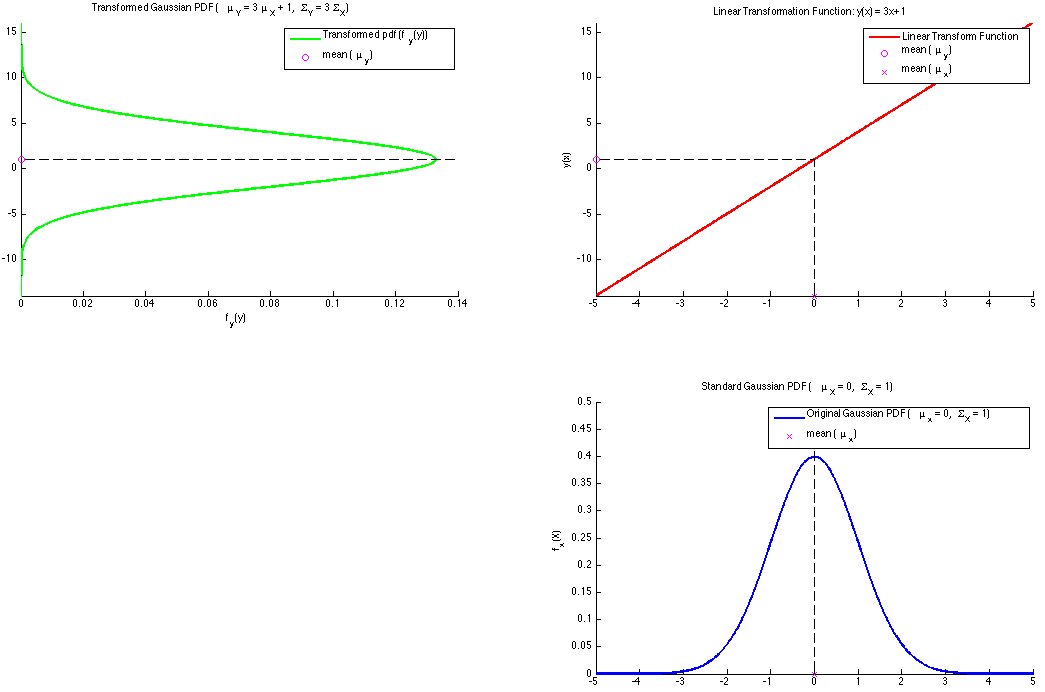
\includegraphics[width=0.49\textwidth, height=0.6\textwidth]{LinTr1.png}
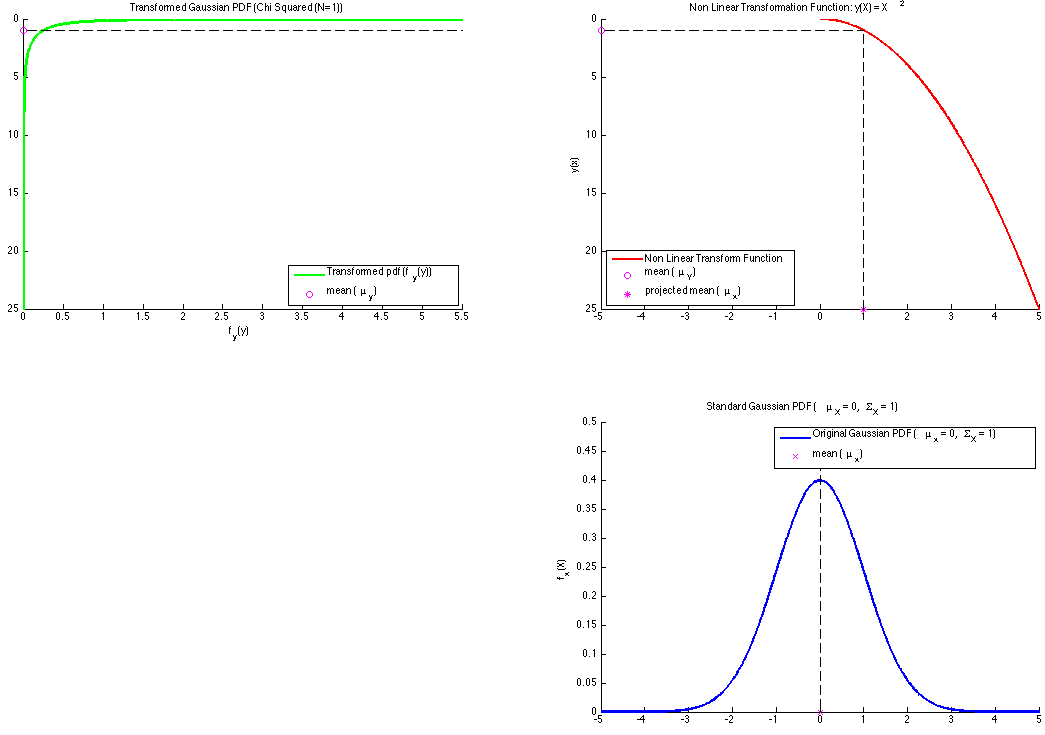
\includegraphics[width=0.49\textwidth, height=0.6\textwidth]{NonLinTr.png}
\caption{Graphical representation depicting both a linear (left) and a non linear (right) transformation of a Gaussian random variable.}
\label{fig:non}
\end{center}
\end{figure}
The \textit{Extended Kalman filter} (EKF), an extension of the general Kalman filter, aims to enable the modelling of non-linear systems through linearisation. As previously mentioned, the state transition function $g(\mu_{t}, {\mu}_{t-1})$, as well as the observation model $h(\bar \mu_t)$ of most practical systems are typically both non-linear in nature. Considering the aforementioned statement; it is necessary to determine a method for approximating a non-linear function as a linear function. The linearisation process of EKF aims to linearise these functions so that the basic fundamental operations of the Kalman Filter algorithm can be validated.\\
The linearisation process approximates an arbitrary non linear function $f$ by a linear function that is \textit{tangent} to $f$ at the mean value of the Gaussian. If the Gaussian is then projected through this new linear approximation, the resultant transformation would yield a random variable that is Gaussian in nature. This technique is applied to both the state transition and observation functions. Many methods exist for linearisation of non linear functions, but the EKF utilises the method of (first order) \textit{Taylor expansion}. The Taylor expansion creates a linear approximation of a non linear function, say $f$, by it's own value as well as that of it's gradient $f'$. The tangent of $f$ can be depicted by it's partial derivative with respect to the state vector $\textbf{x}_{t-1}$:
\begin{equation}\label{eq:par}
f'(\textbf{x}_{t-1}, \textbf{u}_t) := \frac{\partial f(\textbf{x}_{t-1}, \textbf{u}_t)}{\partial \textbf{x}_{t-1}}
\end{equation}
\\
The argument of the function $f$ is chosen as the most likely point at the linearisation instance. For Gaussians, the most likely point is the mean $\mu_{t-1}$. The linear approximation of the function $f$ can then be achieved through the linear extrapolation evaluated at it's most likely point $\mu_{t-1}$:
\begin{equation}\label{eq:app}
\begin{split}
f(\textbf{x}_{t-1}, \textbf{u}_t) &\approx f(\textbf{x}_{t-1}, \textbf{u}_t) + f'(\textbf{u}_{t},\mu_{t-1})(\textbf{x}_{t-1}-\mu_{t-1}) \\
&= f(\textbf{x}_{t-1}, \textbf{u}_t) + \textbf{F}_t(\textbf{x}_{t-1}-\mu_{t-1})
\end{split}
\end{equation}
where $\textbf{F}_t = f'(\textbf{u}_{t},\mu_{t-1})$ is the \textit{Jacobian} matrix. \\
It is important to note that {Jacobian} matrix is determined at each linearisation instance (each individual time-step) as its parameters differ from one linearisation instance to the next. 
\\\\
Once linearisation is achieved, the EKF; which behaves otherwise identically in terms of operation to the general Kalman filter, can be implemented upon non-linear systems. \\
It is very important to note that because only a first order Taylor expansion is used to approximate the linearisation, severe non-linearities will prohibit acceptable approximations of the Gaussian distribution upon transformations. Other variants of the Kalman filter that aren't discussed in this paper, are then required to be considered.\\

Table~\ref{tab:EKF}  below, systematically and mathematically represents the aforementioned steps.

\begin{table}[h]
\begin{center}
\caption{The Extended Kalman Filter Algorithm}\label{tab:EKF}
\begin{tabular}{l l l}
\hline
\textbf{Input}: &previous mean $\mu_{t-1}$ and covariance $\Sigma_{t-1}$, control inputs $\textbf{u}_t$, measurements $\textbf{z}_t$\\ 
\textbf{Output}: &mean $\mu_{t}$, covariance $\Sigma_{t}$\\
\hline
\hline
&\textit{Prediction step} \\
\hline
1. & $\bar \mu_{t}$ = $g(\textbf{u}_t, \mu_{t-1})$ \\
2. & $\bar \Sigma_t = G_t \Sigma_{t-1} G_t^T + R_{w,t}$ \\
\hline
&\textit{Correction step}\\
\hline
3. & $K_t = \bar \Sigma_{t} H_t^T (H_t \bar \Sigma_{t} H_t^T + Q_{v,t})^{-1}$ \\
4. & $\mu_t = \bar \mu_t + K_t[z_t-h(\bar \mu_t)]$\\  
5. & $\Sigma_{t} = (I-K_t H_t)\bar \Sigma_t$ \\
\hline\hline
\end{tabular}
\end{center}
\end{table}%  
%%%%%%%%%%%%%%%%%%%%%%%%%%%%%%%%%%%%%%%%%%%%%%%%%%%%%%%%%%%%%%%%%%%%%%%%%%
\newpage
\section{EKF MonoSLAM: EKF Monocular Based SLAM Using Kinematic State Estimation}
%%%%%%%%%%%%%%%%%%%%%%%%%%%%%%%%%%%%%%%%%%%%%%%%%%%%%%%%%%%%%%%%%%%%%%%%%%
The ultimate goal of the approach presented here, is to obtain a probabilistic three dimensional (3D) map of features, representing at every time instance, the estimates of both the state of the camera as well as the positions of every feature observed. This scenario is typically defined as the SLAM problem. Such a problem, is typically solved through the utilisation of the EKF. The goal of a particular SLAM algorithm termed MonoSLAM (Monocular vision based SLAM), is to ultimately realise the objective of obtaining the aforementioned probabilistic map, through the utilisation of a single camera as achieved by \textcolor{red}{[Davison 2003]}. Various \textbf{successful} SLAM algorithms exist that utilise sensors other than cameras (laser range finders, ultrasonic sensors etc.). Cameras though, prove a better economical alternative to these sensors. Another successful and popular implementation is stereo vision (two calibrated cameras), yet the obvious disadvantage regarding such an approach is that double the cost is required as opposed to a single camera approach.\\  
It can be argued though, that the general approach presented by \textcolor{red}{[Davison 2003]} as well as variants thereof \textcolor{red}{[Other sources]} can be improved through the utilisation of additional information regarding the motion of the robot. The approach presented in this paper then, seeks to utilise exactly such information through the utilisation of an inertial measurement unit (IMU) as an extension to the original implementation. Inertial measurement unit's have been implemented in SLAM based systems before, as implemented in \textcolor{red}{[Other sources]}. With the addition of an IMU, information regarding the changes in movement and orientation of the camera (namely the linear accelerations and the angular rates) can be obtained and \textit{observed} accordingly. Ultimately, the stochastic constant velocity motion model of the general MonoSLAM algorithm can then be replaced with a kinematic estimation based motion model - one that is initially assumed to be more accurate as it contains a considerably larger amount of information. \\ 
Furthermore, the remaining components of the proposed approach presented in this paper are identical to that of the general MonoSLAM algorithm of Davison: that is, using the EKF to successfully obtain the desired probabilistic map. \\\\
This section sets out to define the necessary segments of the MonoSLAM algorithm in the context of this paper alone. Initially the adequate state representation of the system at hand will be denoted, whereby the components of the state vector - namely the camera position and cartesian feature states - will be defined and discussed. Additionally, the affect of the proposed extension - namely the control inputs to the system - will be properly defined and described. Furthermore, this section will seek to use the aforementioned definitions to completely define the two sequential steps required to successfully implement the EKF, namely the prediction and update steps. \\\\
\textcolor{green}{We seek to explain the main idea behind EKF}
\subsection{State Representation}
Generally, a state can be defined as any facet that has the ability to impact the future. In the context of this particular paper, the states will comprise of all facets that impact the future of both the robot and the environment dynamics. As per the definition of the EKF, it is essential that the system possesses a model to estimate future states. This model is commonly referred to as the previously discussed state transition model. All relevant state estimates are embedded within the state vector $\textbf{{x}}_t$, which is comprised of two parts, the camera state $\textbf{{x}}_v$ and the landmark position estimates $\textbf{{y}}$ respectively. The camera state provides the estimate for the robot's pose at each time-step and the landmark estimates provide the landmark's estimated position within the map.\\
Mathematically, the probabilistic map is typically represented through a mean state vector $\textbf{{x}}_t$ and a covariance matrix $\textbf{P}_{nn}$. The mean state vector, as previously mentioned, is a a single column vector containing the estimates of the camera as well as the landmark positions, and $\textbf{P}_{nn}$ is a square matrix containing the covariances of each state with respect to every other state. These quantities can be mathematically shown as follows:
\begin{equation}
\textbf{{x}}_t = 
 \begin{pmatrix}
  \textbf{{x}}_{v,t}\\
  \textbf{{y}}_{1,t} \\ 
  \textbf{{y}}_{2,t} \\
  \vdots \\
  \textbf{{y}}_{n,t}
 \end{pmatrix} , \hspace{0.5cm}
\textbf{P}_{nn} =
 \begin{bmatrix}
  P_{x,x} & P_{x,{y_1}} & P_{x,{y_2}} & \cdots & P_{x,{y_N}} \\
  P_{{y_1},x} &  P_{{y_1},{y_1}} & P_{{y_1},{y_2}} & \cdots &  P_{{y_1},{y_N}} \\
  P_{{y_2},x} &  P_{{y_2},{y_1}} & P_{{y_2},{y_2}} & \cdots &  P_{{y_2},{y_N}} \\
  \vdots  & \vdots  & \vdots & \ddots & \vdots  \\
  P_{{y_n},x} & P_{{y_n},{y_1}} & P_{{y_n},{y_2}}& \cdots & P_{{y_n},{y_n}}
 \end{bmatrix},
\end{equation}
\\These quantities then, allow us to approximate the uncertainty regarding the generated feature map as a $N$-dimensional single multi-variate Gaussian distribution, where $N$, as stated above, is the total number of state estimates within the state vector and $n$ is the total number of landmarks within the map.\\
%%%%%%%%%%%%%%%%%%%%%%%%%%%%%%%%%%%%%%%%%%%%%%%%%%%%%%%%%%%%%%%%%%%%%%%%%%
\subsubsection{Camera Position State Representation}
The following concept describes a suitable method to represent all relevant information regarding the camera's position and orientation in a 3D space. According to most implementations of robot localisation, there exists no contrast between the concepts of a camera state $\textbf{{x}}_v$ and a camera position state $\textbf{x}_p$. It is therefore important to note that a position state - containing the required information regarding a robots position - is merely an element of the camera state vector (where additional information required to describe the camera's position forms the remainder of the camera state vector). The state camera vector - comprising of 10 individual states - is mathematically described as follows:
\begin{equation}
\textbf{{x}}_v=  
 \begin{pmatrix}
  \textbf{{r}}^W\\
  \textbf{{q}}^{WC} \\ 
  \textbf{{v}}^W\\
 \end{pmatrix} ,
\end{equation}
where $\textbf{r}^W =$ (\textit{x} \textit{y} \textit{z}$)^T$ indicates the 3D cartesian position of the camera, $\textbf{{q}}^{WC}$ the unit orientation \textit{quarternion} - to be mathematically defined and described in the appendix - indicating the camera orientation (represented in the body frame $C$) relative to the inertial reference frame $W$ while $\textbf{{v}}^W$ indicates the \textit{linear} velocities of the camera relative to the inertial reference frame $W$.\\Often, the modelling of dynamic systems require that additional parameters - separate to those describing the position and orientation of the robot - be included in the state vector along with the position state vector. This is illustrated in the description above, with the position state vector $\textbf{{x}}_p$ comprising of the 3D position vector, $\textbf{{r}}^W$ and the unit orientation \textit{quarternion}, $\textbf{{q}}^{WC}$. The linear velocity vector, $\textbf{V}^W$, forms the additional information required for system modelling. This is due to the control inputs, which are of such a nature that intermediary states (namely the linear velocity) is required to describe the control inputs effect on the actual position. 
%%%%%%%%%%%%%%%%%%%%%%%%%%%%%%%%%%%%%%%%%%%%%%%%%%%%%%%%%%%%%%%%%%%%%%%%%%
%%%%%%%%%%%%%%%%%%%%%%%%%%%%%%%%%%%%%%%%%%%%%%%%%%%%%%%%%%%%%%%%%%%%%%%%%%   
\subsubsection{Cartesian Feature Representation}
As previously discussed, the aim is to describe a set of high-quality, well defined landmarks within the map. The map itself is to contain a 3D position of \textit{each} observed landmark  as well as a combined uncertainty. The feature estimates $\textbf{{y}}$ - comprising of $N$ landmarks - is mathematically described through three individual cartesian coordinates - $x$, $y$ and $z$ respectively:
\begin{equation}
\textbf{{y}}_n = (x_n\hspace{0.25cm}y_n\hspace{0.25cm}z_n)^T,
\end{equation}
where $n$ corresponds to a specific, single landmark.
%\textcolor{red}{With reference to the theory on image processing, it can be discussed that the depth of a given landmark (in this case the $z$-coordinate) cannot be immediately determined, but rather approximated via triangulation given the landmark is observed over a sequence of (minimally) two known camera positions. The $x$ and $y$ measurements however, can be immediately determined from the image plane.}
%%%%%%%%%%%%%%%%%%%%%%%%%%%%%%%%%%%%%%%%%%%%%%%%%%%%%%%%%%%%%%%%%%%%%%%%%%
\subsubsection{Control Inputs}
%\textbf{Still reading up on some literature before properly defining this section}
The following concept describes the input to the system as a result of external dynamics. Upon considering the approach of \textcolor{red}{[Davison 2003]}, it is evident that there are no \textit{observable} control inputs. The approach presented in this paper though, aims to use observable control inputs that are obtained through inertial sensor to obtain a motion model that is potentially more accurate than that of Davison.\\\\
In most instances of robotics, it is essential to describe the dynamics involving a robot's movement. In the context of this paper, the camera is free to move freely as per the user's control requests. Evidently, these requests exert external dynamics upon the system which are uncertain and stochastic at best.\\
In the approach presented by \textcolor{red}{[Davison 2003]}, a constant velocity model is assumed and at each time-step, unknown linear and angular acceleration zero-mean, Gaussian processes are introduced that cause linear and angular velocity impulses. Even though there have been proven successful implementations regarding the aforementioned approach (as well as other variants and extensions thereof), the model contains very little, if any information on the movement of the camera. It can be assumed that the utilisation of additional information regarding the camera's movement (through inertial sensors) will provide great accuracy upon state estimation - especially with regard to the transitioning thereof.\\\\
The inertial sensors, in the form of an IMU, is ideally be mounted onto the camera. This allows the camera to be modelled as a rigid body upon which a kinematic estimation can be applied. The IMU directly measures the total accelerations $\textbf{f}_t$ as well as the angular rates $\mathbf{\omega}_t$ with respect to the cameras rigid body frame $C$.\\ 
The control vector however, requires that the linear portion of the acceleration be obtained from the IMU measurement. It is known that the total acceleration measured by the IMU's accelerometer is expressed mathematically as follows:

\begin{equation}
\textbf{f}_t = \textbf{R}(\textbf{a}_t - \textbf{g}_t)
\end{equation}
where $\textbf{R}$ is the rotation matrix that transforms the body coordinate frame data into the inertial reference frame, $\textbf{a}_t$ is the linear acceleration vector and $\textbf{g}_t$ is the gravity vector. \\
Once obtained, these measurements (not to be confused with the EKF's measurements) form the control vector $\textbf{u}_t$ that describes, at each time-step, the dynamics of the system as a result of external forces. The control vector is mathematically described as follows:

\begin{equation}
\textbf{u}_t =
\begin{pmatrix} 
 \textbf{a}_t \\
 {\omega}_t
\end{pmatrix}
= \big[\hspace{0.1cm}\ddot{x}_{t}\hspace{0.25cm}\ddot{y}_{t}\hspace{0.25cm}\ddot{z}_{t}\hspace{0.25cm}\textit{\.{q}}_{0,t}\hspace{0.25cm}\textit{\.{q}}_{1,t}\hspace{0.25cm}\textit{\.{q}}_{2,t}\hspace{0.25cm}\textit{\.{q}}_{3,t}\hspace{0.1cm}\big]^T
\end{equation}
Because the IMU measurements gather the actual data through exteroceptive sensors, namely an accelerometer and a gyroscope, it is important to note the effects of disturbances and process noise can be directly obtained through these measurements. Moreover, the uncertainty regarding the transition model, namely the process noise, is all incorporated within the noise measurements of the IMU. This noise can be modelled as a zero mean, Gaussian process $\textbf{w}_t$ with a corresponding covariance matrix $\textbf{R}_w$. The system noise can be then be mathematically described as follows:
 
\begin{equation}
\textbf{w}_t =
\begin{pmatrix} 
 \textbf{n}_{\textbf{a},t} \\
 \textbf{n}_{{\omega},t}
\end{pmatrix}
= \big[\hspace{0.1cm}n_{\ddot{x}_{k}}\hspace{0.25cm}n_{\ddot{y}_{k}}\hspace{0.25cm}n_{\ddot{z}_{k}}\hspace{0.25cm}n_{\textit{\.{q}}_{0,k}}\hspace{0.25cm}n_{\textit{\.{q}}_{1,k}}\hspace{0.25cm}n_{\textit{\.{q}}_{2,k}}\hspace{0.25cm}n_{\textit{\.{q}}_{3,k}}\hspace{0.1cm}\big]^T
\end{equation}
where the aforementioned noise model yielding each of the above elements a Gaussian random variable.  \\
Furthermore, the resultant IMU data to be used are to contain the measurements of the linear accelerations and angular rotations as well as the appropriate additive noise.
%%%%%%%%%%%%%%%%%%%%%%%%%%%%%%%%%%%%%%%%%%%%%%%%%%%%%%%%%%%%%%%%%%%%%%%%%%
\subsection{Prediction Step}
With reference to the probabilistic form of the solution to the SLAM problem, the prediction step requires a description in terms of a belief distribution. The description of the aforementioned state transition model can then, in terms of the probability distribution on the state transitions, take the following form:
\begin{equation}
\begin{split}
bel(\textbf{x}_t) &= p(\textbf{{x}}_t\hspace{0.15cm}|\hspace{0.15cm}\textbf{{x}}_{t-1}, \textbf{u}_t) \\
&=\cfrac{1}{\sqrt{|2\pi\textbf{R}_w|}}\hspace{0.1cm}\text{exp}\hspace{0.1cm}\bigg\{ \frac{1}{2}\big[\textbf{{x}}_t-g(\mu_t, \hspace{0.1cm}\mu_{t-1}) - G_t(\textbf{x}_{t-1} - \mu_{t-1})\big]^T\\
&\textbf{R}^{-1}_w\big[\textbf{{x}}_t-g(\mu_t, \hspace{0.1cm}\mu_{t-1}) - G_t(\textbf{x}_{t-1} - \mu_{t-1})\big]\bigg \},
\end{split}
\end{equation} 
where $G_t$ represents the Jacobian of the state transition motion. \\\\
The state transition model is assumed to take the form of a Markov process, yielding that the current state $\textbf{{x}}_{t}$ is only dependent upon the state immediately preceding it - $\textbf{{x}}_{t-1}$ - as well as the input control $\textbf{{u}}_t$. Additionally, it is important to note that the uncertainty regarding the state transition model is independent of the uncertainty regarding both the observation model as well as that of the probabilistic map itself.
%%%%%%%%%%%%%%%%%%%%%%%%%%%%%%%%%%%%%%%%%%%%%%%%%%%%%%%%%%%%%%%%%%%%%%%%%%

%%%%%%%%%%%%%%%%%%%%%%%%%%%%%%%%%%%%%%%%%%%%%%%%%%%%%%%%%%%%%%%%%%%%%%%%%%

\subsubsection{State Transition Model} 
As previously discussed, the Extended Kalman FiIter requires a state transition (motion) model in order to estimate the current state of the system. In short, the motion model describes the transition from the previous state to the following state with regard to the robot�s kinematic motion as well as the control inputs. In order to derive the state transition model for the system at hand, it is vital that the certain characteristics of the system be understood. Firstly, the robot system - from here on in to be referred to as the \textbf{camera} - is comprised of a monocular camera and an attached Inertial Measurement Unit (IMU) package. Secondly, the camera is to be considered as a six degree of freedom (DOF) rigid body. Briefly the six DOF describe the camera's three \textit{translational} and three \textit{rotational} degrees of freedom. \\\\
We therefore set out to define a kinematic motion model - using Newton's laws of motion - to describe the cameras movement through the environment as a result of initially unknown, external inputs to the system. Lastly, it should be stressed that embedded within the motion model, should be the impacts of uncertainty through both internal and external factors.\\
It must also be stressed that initially, a stochastic, non linear discrete-time model is adopted to approximate the model. We begin by describing all relevant states and control inputs:
\begin{equation}
\begin{split}
\textbf{x}_t &=\big[\hspace{0.1cm}\textbf{r}_t^{W}\hspace{0.1cm}\textbf{q}_t^{WC}\hspace{0.1cm}\textbf{v}_t^{W}\big]^T\\ 
&= \big[\textit{x}_{t}\hspace{0.25cm}\textit{y}_{t}\hspace{0.25cm}\textit{z}_{t}\hspace{0.25cm}\textit{\.{x}}_{t}\hspace{0.25cm}\textit{\.{y}}_{t}\hspace{0.25cm}\textit{\.{z}}_{t}\hspace{0.05cm}\hspace{0.25cm}\textit{q}_{0,t}\hspace{0.25cm}\textit{q}_{1,t}\hspace{0.25cm}\textit{q}_{2,t}\hspace{0.25cm}\textit{q}_{3,t}\big]^T \\
\textbf{u}_t &= \big[\hspace{0.1cm}\textbf{a}_t^C\hspace{0.1cm}\dot{\omega}_t^C\big]^T\\
&=\big[\hspace{0.1cm}\ddot{x}_{t}\hspace{0.25cm}\ddot{y}_{t}\hspace{0.25cm}\ddot{z}_{t}\hspace{0.25cm}\textit{\.{q}}_{0,t}\hspace{0.25cm}\textit{\.{q}}_{1,t}\hspace{0.25cm}\textit{\.{q}}_{2,t}\hspace{0.25cm}\textit{\.{q}}_{3,t}\big]^T\\
\end{split}
\end{equation}
The state transition function $g_v(\textbf{u}_{t},\mu_{t-1})$ is defined as follows:
\begin{equation}
\begin{split}
g_v(\textbf{u}_{t},\mu_{t-1}) =
	\begin{pmatrix}
		\textbf{r}_t^{W}\\
		\textbf{q}_t^{WC}\\
		\textbf{v}_t^{W} \\
	\end{pmatrix} &= 
	\begin{pmatrix}
		\textbf{r}_{t-1}^{W}+\textbf{v}_t^W\Delta T\\
		\textbf{q}_{t-1}^{WC} \otimes \text{quat}\big(\dot{\omega}_t^C\Delta T\big) \\
		\textbf{v}_t^{W} + \textbf{a}_{t}^C \Delta T \\
	\end{pmatrix} \\
&= \begin{pmatrix}
	 \textbf{r}_{t-1}^{W}+\dot{\textbf{r}}^W\Delta T\\
	 \textbf{q}_{t-1}^{WC} \otimes \text{quat}\big(\textbf{\.{q}}_t^C\Delta T\big) \\
	 \dot{\textbf{r}}_t^{W} + \textbf{R}_t^{CW}\big(\ddot{\textbf{r}}_{t}^C \Delta T\big) \\
\end{pmatrix}
\end{split}
\end{equation}
%%%%%%%%%%%%%%%%%%%%%%%%%%%%%%%%%%%%%%%%%%%%%%%%%%%%%%%%%%%%%%%%%%%%%%%%%%
\newpage
\subsection{Correction Step}
With reference again to the probabilistic form of the solution to the SLAM problem, the measurement step too, requires a description in terms of a probability distribution. The observation model however, models the uncertainty regarding a measurement taken at an instance $\textbf{{z}}_t$ given that the locations of both the robot as well as the landmarks are known. This uncertainty can be described in the following form:  
\begin{equation}
\begin{split}
P(&\textbf{z}_t\hspace{0.1cm}|\hspace{0.15cm}\textbf{x}_{t}) \\
&=\cfrac{1}{\sqrt{|2\pi\textbf{Q}_t|}}\hspace{0.1cm}\text{exp}\hspace{0.1cm}\Big\{ \frac{1}{2}\big[\textbf{{z}}_t-h(\bar \mu)-H_t(\textbf{x}_t - \bar \mu_t)\big]^T \textbf{Q}_t^{-1}\big[\textbf{{z}}_t-h(\bar \mu)-H_t(\textbf{x}_t - \bar \mu_t)\big] \Big\}.
\end{split}
\end{equation} 
where $H_t$ represents the Jacobian of the observation model. \\\\
It can be (reasonably) assumed that the uncertainty regarding the measurements are conditionally independent given the uncertainty regarding the robot and landmark locations if indeed they are completely defined. Also, the correction step seeks to obtain the difference between the actual measurements $\textbf{\^{z}}_k$ and the predicted measurements. These predicted measurements are to be obtained through an observation model that we from hereon in refer to as the measurement function, denoted as $\textbf{h}_i$.  
%%%%%%%%%%%%%%%%%%%%%%%%%%%%%%%%%%%%%%%%%%%%%%%%%%%%%%%%%%%%%%%%%%%%%%%%%%
\subsubsection{Measurement Function}
The correction step of the Extended Kalman filter aims to ultimately correct the previously estimated robot pose and landmark position through exterior sensor measurements. The measurement process generally involves a measurement estimate that incorporates an uncertainty. With regard to the implantation proposed in this paper, landmarks are required to be observed and measured through the use of a camera. To mathematically describe this process, the previously mentioned measurement function is used to effectively model the measurement estimation. It is essential that the measurement function, like the motion model, be \textbf{linear} in nature and additionally, the measurement function {must} describe the position of a \textbf{point} feature with regard to the previously estimated states - namely the robot pose and the landmark positions. \\\\   
Considering that the camera observations are obtained with regard to its own reference frame $C$, the definition of the measurement function is adapted in order to be described with regard to the inertial reference frame. The measurement function $\textbf{h}^W_i$ that describes a directional vector in relation to the cameras body frame is thus mathematically defined as follows: 
\begin{equation}
\textbf{h}^W_i = \textbf{R}^{CW}\big(\textbf{y}^W_i-\textbf{r}^W\big) = 
  \begin{pmatrix}
  \begin{pmatrix}
  x_i\\
  y_i \\ 
  z_i \\
  \end{pmatrix} - \textbf{r}^{W} 
  \end{pmatrix}  
\end{equation}
where the subscript $i$ corresponds a directional vector $\textbf{h}^C$ to its cartesian point $\textbf{y}^W$, $\textbf{r}^W$ describes the cartesian position of the camera, $\textbf{y}^W$ describes the cartesian position of a given landmark and $\textbf{R}^{CW}$ represents the rotational matrix that is required to transform the aforementioned positional vectors from the inertial reference frame into the cameras body frame coordinate system.\\\\
With reference to the section regarding perspective cameras, it can be recalled that a given features position is described by a 2-dimensional position of the image frame of the camera. Recalling, the standard pinhole camera model defines this position mathematically as follows:
 \begin{equation}
\textbf{h}_i = 
  \begin{pmatrix}
  u_i\\
  v_i \\ 
  \end{pmatrix} =
    \begin{pmatrix}
  u_0 - fk_u\frac{h^R_{i,x}}{h^R_{i,z}}\\
  v_0 - fk_v\frac{h^R_{i,y}}{h^R_{i,z}} \\ 
  \end{pmatrix} 
\end{equation}
where $fk_u$, $fk_v$, $u_0$ and $v_0$ are the previously described camera calibration parameters.\\


%%%%%%%%%%%%%%%%%%%%%%%%%%%%%%%%%%%%%%%%%%%%%%%%%%%%%%%%%%%%%%%%%%%%%%%%%%
\subsubsection{Feature Tracking}
%%%%%%%%%%%%%%%%%%%%%%%%%%%%%%%%%%%%%%%%%%%%%%%%%%%%%%%%%%%%%%%%%%%%%%%%%%
\subsubsection{System Update}
%%%%%%%%%%%%%%%%%%%%%%%%%%%%%%%%%%%%%%%%%%%%%%%%%%%%%%%%%%%%%%%%%%%%%%%%%%
%%%%%%%%%%%%%%%%%%%%%%%%%%%%%%%%%%%%%%%%%%%%%%%%%%%%%%%%%%%%%%%%%%%%%%%%%%
%%%%%%%%%%%%%%%%%%%%%%%%%%%%%%%%%%%%%%%%%%%%%%%%%%%%%%%%%%%%%%%%%%%%%%%%%%
%%%%%%%%%%%%%%%%%%%%%%%%%%%%%%%%%%%%%%%%%%%%%%%%%%%%%%%%%%%%%%%%%%%%%%%%%%
%%%%%%%%%%%%%%%%%%%%%%%%%%%%%%%%%%%%%%%%%%%%%%%%%%%%%%%%%%%%%%%%%%%%%%%%%%
%%%%%%%%%%%%%%%%%%%%%%%%%%%%%%%%%%%%%%%%%%%%%%%%%%%%%%%%%%%%%%%%%%%%%%%%%%
%%%%%%%%%%%%%%%%%%%%%%%%%%%%%%%%%%%%%%%%%%%%%%%%%%%%%%%%%%%%%%%%%%%%%%%%%%
%%%%%%%%%%%%%%%%%%%%%%%%%%%%%%%%%%%%%%%%%%%%%%%%%%%%%%%%%%%%%%%%%%%%%%%%%%
%%%%%%%%%%%%%%%%%%%%%%%%%%%%%%%%%%%%%%%%%%%%%%%%%%%%%%%%%%%%%%%%%%%%%%%%%%
 














\newpage
\appendix
\section{Linear State Space Model} \label{App:AppendixA}
\subsection{State Space Model} 
As previously discussed, the Extended Kalman FiIter requires a state transition (motion) model in order to estimate the current state of the system. In short, the motion model describes the transition from the previous state to the following state with regard to the robot's kinematic motion as well as the control inputs. The \textit{ideal} motion model in this particular instance can be described through a \textbf{linear} differential equation of the following form:
\begin{equation}
\textbf{\.{x}}_t = \textbf{A}\textbf{x}_{t-1} + \textbf{B}\textbf{u}_t+\textbf{w}_t,
\end{equation} 
where the state matrix $\textbf{A}$, describes the manner in which state evolves from the previous time-step to the current time-step without the influence of noise and controls, the input matrix $\textbf{B}$, describes how the control vector $\textbf{u}_t$ evolves from the previous time-step to the current time-step and $\textbf{w}_t$ is a \textbf{zero-mean} Gaussian process representing the process noise with a covariance matrix $\textbf{R}_w$.\\\\
Considering that the Extended Kalman Filter is a recursive, numerical evaluation, it is necessary to convert the previously defined continuous model into its discrete counterpart. Various methods of discretisation exist, though this specific implementation makes use of the forward difference/Euler�s method. This method  \textit{approximates} the derivative for a state for a sampling period $\Delta T$ as follows:  
\begin{equation}
\begin{split}
\textbf{\.{x}}_k &= \lim_{\Delta T\to 0}{\frac{\textbf{x}_{k+1}-\textbf{x}_k}{\Delta T}} 		 \\										\Delta T\textbf{\.{x}}_k &\approx \textbf{x}_{k+1}-\textbf{x}_k, \\
\end{split}
\end{equation}     
The state estimate of the discrete counterpart at the following sampling instance, namely $k + 1$, is then presented as follows (given a small enough sampling instance $\Delta T$):
\begin{equation}
\begin{split}
\textbf{x}_{k+1} &= \big(\textbf{I}+\textbf{A}\Delta T\big)\textbf{x}_k + \textbf{B}\textbf{u}_k\Delta T + \textbf{w}_k\Delta T,
\end{split}
\end{equation}
where $\big(\textbf{I}+\textbf{A}\Delta T\big) = \textbf{A}_d$ is the discrete state matrix, $ \textbf{B}\Delta T = \textbf{B}_d$ is the discrete input matrix and $\textbf{w}_k\Delta T=\textbf{w}_{d,k}$ is the discrete input process noise. \\\\
Ultimately, the form of the final difference equation describing the system at each individual sampling instance is given as follows:
\begin{equation}
\textbf{x}_{k+1}= \textbf{A}_d\textbf{x}_k + \textbf{B}_d\textbf{u}_k+\textbf{w}_{d,k},
\end{equation} 

\subsection{State Transition: Linear Model}
In order to derive the motion model for the system at hand, it is vital that the certain characteristics of the system be understood. Firstly, the robot system - from here on in to be referred to as the \textbf{camera} - is comprised of a monocular camera and an attached Inertial Measurement Unit (IMU) package. Secondly, the camera is to be considered as a six degree of freedom (DOF) rigid body. Briefly the six DOF describe the camera's three \textit{translational} and three \textit{rotational} degrees of freedom. \\
We therefore set out to define a kinematic motion model - using Newton's laws of motion - to describe the cameras movement through the environment as a result of initially unknown, external inputs to the system. Lastly, it should be stressed that embedded within the motion model, should be the impacts of uncertainty through both internal and external factors. 
%It is assumed in this instance, that at each time-step, an unknown angular acceleration $\mathbf{\Omega}^R$ acts upon the system. This input is modelled as a zero-mean Gaussian process that causes an impulse of angular velocity:
%\begin{equation}
%\textbf{w}_d[k]  = \textbf{w}[k] \Delta T =     
% \begin{bmatrix}
% \mathbf{\Omega}^R
% \end{bmatrix} = 
%  \begin{pmatrix}
%  	\alpha_x \Delta T \\
% 	\alpha_y \Delta T \\
%\alpha_z \Delta T \\
% \end{pmatrix} .
%\end{equation}  
%with a covariance matrix $\textbf{R}_w$ that is assumed as a diagonal initially, to represent uncorrelated noise in all of the rotational components.\\
%With reference to the previously defined state motion model in (1.8)
It must also be stressed that initially, a stochastic, linear discrete-time model is adopted to approximate the motion model. Using the kinematic equations of linear and angular motion, it is aimed to ultimately and complete the previously defined state space model. We begin by describing all relevant states and control inputs:
\begin{equation}
\begin{split}
\textbf{x}[k] &= \big[\textit{x}_{k}\hspace{0.25cm}\textit{y}_{k}\hspace{0.25cm}\textit{z}_{k}\hspace{0.25cm}\textit{\.{x}}_{k}\hspace{0.25cm}\textit{\.{y}}_{k}\hspace{0.25cm}\textit{\.{z}}_{k}\hspace{0.05cm}\hspace{0.25cm}\textit{q}_{0,k}\hspace{0.25cm}\textit{q}_{1,k}\hspace{0.25cm}\textit{q}_{2,k}\hspace{0.25cm}\textit{q}_{3,k}\big]^T \\
\textbf{u}[k] &= \big[\hspace{0.1cm}\ddot{x}_{k}\hspace{0.25cm}\ddot{y}_{k}\hspace{0.25cm}\ddot{z}_{k}\hspace{0.25cm}\textit{\.{q}}_{0,k}\hspace{0.25cm}\textit{\.{q}}_{1,k}\hspace{0.25cm}\textit{\.{q}}_{2,k}\hspace{0.25cm}\textit{\.{q}}_{3,k}\big]^T\\
\end{split}
\end{equation}
and extend the discrete-time difference equation describing the system to incorporate the motion model,  
\begin{equation}
\begin{split}
\textbf{x}_{k+1} &= \textbf{A}_d\textbf{x}_k + \textbf{B}_d\textbf{u}_k+\textbf{w}_{d,k}, \\
\textbf{A}_d&= 
 \begin{bmatrix}
  1 & 0 & 0 & \Delta T & 0 & 0 & 0 & 0 & 0 & 0 \\
  0 & 1 & 0 & 0 & \Delta T & 0 & 0 & 0 & 0 & 0 \\
  0 & 0 & 1 & 0 & 0 & \Delta T & 0 & 0 & 0 & 0 \\
  0 & 0 & 0 & 1 & 0 & 0 & 0 & 0 & 0 & 0 \\
  0 & 0 & 0 & 0 & 1 & 0 & 0 & 0 & 0 & 0 \\
  0 & 0 & 0 & 0 & 0 & 1 & 0 & 0 & 0 & 0 \\
  0 & 0 & 0 & 0 & 0 & 0 & 1 & 0 & 0 & 0 \\
  0 & 0 & 0 & 0 & 0 & 0 & 0 & 1 & 0 & 0 \\
  0 & 0 & 0 & 0 & 0 & 0 & 0 & 0 & 1 & 0 \\
  0 & 0 & 0 & 0 & 0 & 0 & 0 & 0 & 0 & 1 \\
 \end{bmatrix} = (\textbf{I}+\textbf{A}\Delta T\big),  \\
 \textbf{B}_d&=
\begin{bmatrix}
  \Delta T & 0 & 0 & 0 & 0 & 0 & 0 \\
  0 & \Delta T & 0 & 0 & 0 & 0 & 0 \\
  0 & 0 & \Delta T & 0 & 0 & 0 & 0 \\
  0 & 0 & 0 & \Delta T & 0 & 0 & 0 \\
  0 & 0 & 0 & 0 & \Delta T & 0 & 0 \\
  0 & 0 & 0 & 0 & 0 & \Delta T & 0 \\
  0 & 0 & 0 & 0 & 0 & 0 & \Delta T \\
\end{bmatrix} = \textbf{B}\Delta T, \\\\
 \textbf{w}_{d,k} &=\mathcal{N}(0,  \textbf{R}_w) =  
 \begin{pmatrix}
 \textbf{n}_{\textbf{a}_t,k} \\
 \textbf{n}_{\omega_t,k} \\
 \end{pmatrix} = \textbf{w}_{d,k} \Delta T, 
 \end{split}
\end{equation}
it can be observed from the model above that the motion model adheres to the forward method of discretisation derived in (2.8). The motion model also adheres to the Markov process assumption, in that it can be completely described through only its transition from the previous state as well as the control inputs.   

  %\begin{bmatrix}
  %x_k\\
  %y_k \\ 
  %z_k \\
  %q_{0,k}\\
  %q_{1,k}\\
  %q_{2,k}\\
  %q_{3,k}\\
  %\dot{x}_k\\
  %\dot{y}_k\\
  %\dot{z}_k\\
  %\end{bmatrix}  
  %The position state $\textbf{{x}}_p$ can furthermore be fully represented as follows:
%\begin{equation}
%\textbf{{x}}_p=  
% \begin{pmatrix}
% x\\
% y\\ 
% z\\
% q_0\\
% q_1\\
% q_2\\
% q_3\\
% \end{pmatrix} .
%\end{equation}  
%Various alternative implementations exist to represent a robots pose in a 3D space, each presenting their own unique advantages (and disadvantages) with respect to the others. A representation of an arbitrary 3D position and orientation, requires at least, three parameters describing the cartesian position as well as an additional three describing the orientation. This specific implementation, utilises the \textbf{quarternion} representation to portray the orientation information and thus requires an additional parameter to aid its description. 

%This description then allows for the implementation of a recursive algorithm, namely, a discrete Kalman filter. In order for a Kalman filter to be successfully implemented, a \textbf{state transition (motion) model} as well as an \textbf{observation model} is required to individually describe the effects of the control input as well as the observations respectively.\\
%It is important to note that the Kalman filter estimates the state of a continuous- or discrete-time process that is described by a set of differential (continuous) or difference (discrete) equations. The Kalman filter then continuously updates the state estimates according to the measurements it obtains. This procedure, takes the form of a two-step recursive process: an a priori prediction (time-update) and an observation based correction (measurement-update). 


\end{document}   